\documentclass{article}
\newcommand{\mod}[1]{\texttt{#1}}
\usepackage{natbib}
\usepackage{graphicx}
\bibliographystyle{plainnat}
\usepackage{fancyheadings}
\usepackage{tabularx}
\usepackage{alltt, parskip, boxedminipage}
\usepackage{makeidx, multirow, longtable, tocbibind, amssymb}
%\usepackage{fullpage}
\makeindex
\usepackage[usenames]{color}
\definecolor{darkblue}{rgb}{0,0.05,0.35}

\usepackage[dvips, pagebackref, pdftitle={}, pdfcreator={epydoc 2.1}, bookmarks=true, bookmarksopen=false, pdfpagemode=UseOutlines, colorlinks=true, linkcolor=black, anchorcolor=black, citecolor=black, filecolor=black, menucolor=black, pagecolor=black, urlcolor=darkblue]{hyperref}
\setlength{\textheight}{21.5cm}
\setlength{\textwidth}{18cm}
\setlength{\hoffset}{-3.0cm}
\setlength{\footskip}{1.5cm}
\setlength{\headsep}{2.5cm}
\setlength{\voffset}{-2.5cm}
\newlength{\BCL} % base class length, for base trees.

\usepackage{everyshi}
 \makeatletter
 \let\totalpages\relax
 \newcounter{mypage}
 \EveryShipout{\stepcounter{mypage}}
 \AtEndDocument{\clearpage
    \immediate\write\@auxout{%
     \string\gdef\string\totalpages{\themypage}}}
 \makeatother

\newcommand{\esofooter}{

\includegraphics[height=1cm]{durlogo.eps}
{\bf \large Centre for \AA dvanced Instrumentation}
}
\newcommand{\esoheaderl}{

\includegraphics[height=1cm]{durlogo.eps}
\begin{tabularx}{9cm}{c}
\Large {\bf \esotitle} \\ \large {\bf(\esodoctype)}\\
\rightmark\hspace{0.1cm}
\end{tabularx}
\vfill
}
\newcommand{\esoheaderc}{
}
\newcommand{\esoheaderr}{
\begin{tabular}{|l|l|}\hline
Doc. number: & \esodocno \\ \hline
Release date: & \esoreleasedate \\ \hline
Issue number: & \esoissue \\ \hline
Page number: & Page \thepage \ of \totalpages \\ \hline
Author(s) & \esoauthorname \\ \hline
\end{tabular}


}

\pagestyle{fancy}
\cfoot[]{}
\lfoot[\esofooter]{\esofooter}
\lhead[\esoheaderl]{\esoheaderl}
\chead[\esoheaderc]{\esoheaderc}
\rhead[\esoheaderr]{\esoheaderr}
\renewcommand{\sectionmark}[1]{\markboth{#1}{#1}}

\newenvironment{Ventry}[1]%
  {\begin{list}{}{%
    \renewcommand{\makelabel}[1]{\texttt{##1:}\hfil}%
    \settowidth{\labelwidth}{\texttt{#1:}}%
    \setlength{\leftmargin}{\labelsep}%
    \addtolength{\leftmargin}{\labelwidth}}}%
  {\end{list}}


\begin{document}
\newcommand{\daspproject}{AO Simulation Project}
\newcommand{\dasptitle}{AO Simulation overview}
\newcommand{\daspdocno}{AOSIM-OVR-UoD-001}
\newcommand{\daspdoctype}{Internal}
\newcommand{\daspissue}{0.1.1}
\newcommand{\daspreleasedate}{\today}
\newcommand{\daspauthorname}{Alastair Basden}
\newcommand{\daspauthortype}{AO sim team member}
\newcommand{\daspapprovername}{Alastair Basden}
\newcommand{\daspapprovertype}{AO sim team member}
\newcommand{\daspreleasername}{Alastair Basden}
\newcommand{\daspreleasertype}{AO sim team member}
\newcommand{\daspreviewername}{Alastair Basden}
\newcommand{\daspreviewertype}{AO sim team member}
\newcommand{\daspchangerecord}{
\begin{tabular}{|l|l|l|l|}
\hline
Issue number & Release date & section(s) affected & Description of
change/remarks\\ \hline
0.1.0 & 051111 & All & First draft \\ \hline
0.1.1 & 051111 & All & Corrections made to first draft\\ \hline
\end{tabular}
}
\newcommand{\daspnotificationlist}{
Alastair Basden\\
Francois Assemat\\
Richard Wilson\\
Tim Morris\\
Tim Butterley\\
Ali Bharmal\\
}
\newcommand{\daspabbreviations}{
\begin{tabular}{rl}
AO & Adaptive Optics\\
ESO & European Southern Observatory\\
\end{tabular}
}
\newcommand{\daspapplicabledocs}{
\begin{tabular}{|l|l|l|}\hline
AD Number & Document title & Doc number/publication/location \\ \hline
AD01 & Simulation API document & AOSIM-API-UoD-001\\ \hline
AD02 & Simulation for dummies document & AOSIM-DUM-UoD-001\\ \hline
\end{tabular}
}
\newcommand{\dasprefdocs}{
\begin{tabular}{|l|l|l|}\hline
RD number & Document title & Doc number/publication/location \\ \hline
RD01 & Durham FPGA website & www.durham.ac.uk/rtcs.project \\ \hline
\end{tabular}
}
\title{\dasptitle}



\thispagestyle{empty}
%This next command provides the CVS tag.  If you want a cvs tag on
%your document, add the following line at the start of the document,
%after replacing the & signs with dollar signs...
%\newcommand{\cvsID}{& &Id& (CVS)&}
\providecommand{\cvsID}{CVS ID not provided: document made on \today}

\begin{center}

\includegraphics{durlogo.eps}
\end{center}
\vspace{0.5cm}
\Huge
\begin{center}
\esoproject\\
\end{center}
\Large
\vspace{1cm}


{\bf 
\begin{tabular}{ll}
Document title: & \esotitle \vspace{0.5cm}\\ 

Documentation number: & \esodocno \vspace{0.5cm}\\ 

Document type: & \esodoctype \vspace{0.5cm}\\ 

Issue number:& \esoissue \vspace{0.5cm}\\ 

Release date: & \esoreleasedate \\ 

\end{tabular}
}

\normalsize
\vfill

\begin{tabular}{|l|l|l|p{5cm}|}
\hline
Document & \esoauthorname & Signature &\\
prepared by & \esoauthortype & and date &\\ \hline
Document & \esoapprovername & Signature &\\
approved by & \esoapprovertype & and date &\\ \hline
Document & \esoreleasername & Signature &\\
released by & \esoreleasertype & and date &\\ \hline
Document & \esoreviewername & Signature &\\
reviewed by & \esoreviewertype & and date &\\ \hline
\end{tabular}

\small
%\begin{alltt}
\cvsID
%\end{alltt}
\normalsize
%\lfoot[\esofooter]{\esofooter}
%\lhead[\esoheaderl]{\esoheaderl}
%\chead[\esoheaderc]{\esoheaderc}
%\rhead[\esoheaderr]{\esoheaderr}
%\renewcommand{\sectionmark}[1]{\markboth{#1}{#1}}

\pagebreak



\begin{center}
\Large
{\bf Change record\\ \vspace{1cm}}
\normalsize
\esochangerecord
\end{center}
\vspace{2cm}

\begin{center}
\Large
{\bf Notification list\\ \vspace{1cm}}
\normalsize
\esonotificationlist
\end{center}

\pagebreak

\begin{center}
\Large
{\bf Acronyms and abbreviations\\ \vspace{1cm}}
\normalsize
\esoabbreviations
\end{center}

\pagebreak

\begin{center}
\Large
{\bf Applicable documents\\ \vspace{1cm}}
\normalsize

\esoapplicabledocs
\end{center}
\vspace{2cm}

\begin{center}
\Large
{\bf Reference documents \\ \vspace{1cm}}
\normalsize

\esorefdocs
\end{center}

\pagebreak
\tableofcontents
\pagebreak

\section{Scope}
This document describes the details of AO simulation software package
which is funded by the rolling grant.

This document is relevant to anyone who is involved with the
development of the AO simulation software.  For a brief description on
how to set up your own AO simulation, please read \citet{dummies}.
\subsection{Bug notification}
Please note, Python 2.5/Numeric combination have a bug:
\begin{verbatim}
a=Numeric.zeros((10,),''d'')
print a[5:].shape
\end{verbatim}
You would hope for this to return (5,) not (0,).  The fix is to add a
comma between the colon and bracket, i.e.\ \texttt{[5:,]}.  I think
this has been done for most of the simulation, but if you encounter
strange bugs that could be related to this, please let me know.  The
simulation has now been converted to numpy, so this should not be an issue.


\subsection{Overview}

The AO simulation package is to be used to simulate the effect of
atmospheric turbulence on large astronomical telescopes.  It has been
designed in such a fashion that it is modular, and so extensible
should future requirements change.  Each module is designed to perform
a specific simulation task, and are connected together by the user in
such a way that coherent results will be obtained from the simulation.

These modules communicate with each other by passing data, either
within their process, using shared memory, or using MPI message
passing.  The simulation framework has been designed so that this
method of message passing is more or less transparent to the user,
with the exception that the user should place the required
communication protocol modules in the correct place.

Additionally, there is a library of useful utilities which the
framework objects use.  The AO simulation package can be treated as
two separate components: One, a library of utilities, including
centroid libraries, science image libraries etc, and two, a simulation
framework complete with simulation objects just waiting to be tied
together and run.  As time allows, it is hoped that more and more of
these simulation framework science objects will move their core
algorithms into the science libraries, and call these.  This will
allow the library to be used in situations where the whole framework
is not ideal.

\subsubsection{Module design}
A user of the simulation software will often wish to simulate some
novel feature which will require development of specific simulation
modules.  When designing a module, certain rules can be followed to
ensure that this module is compatible with the rest of the simulation.
These rules are defined in this document.

The simulation can be set up using a GUI (see simsetup.pdf), which
allows the user to create links between modules.  The simulation can
then be run, and a GUI can be attached or detached at any time to
allow the user to view or debug the simulation at that particular
point.

\subsection{Simulation software modules}
Simulation modules are connected together and provide and get data
as and when it is required.  An example of this is shown in
Fig.~\ref{fig:modules}

\begin{figure}
\includegraphics[height=5cm]{pics/example.eps}
\caption{A figure showing the data flow between connected simulation
  modules.}
\label{fig:modules}
\end{figure}

Each module object is written as an extension to the aobase module
provided in the simulation package.  These objects should always
overwrite the \texttt{generateNext()} method.  During object
initialisation, the object is passed a reference to a predecessor
object (in the example shown in Fig.~\ref{fig:modules}, the
predecessor of the atmos object will be the mkscrns object), and when
the object requires data from it's predecessor, it finds it in
\texttt{self.parent.outputData}.  If the object is to alter this data,
it should make its own copy. 

Once an object's generateNext() method has completed, the object will
have placed it's output in the \texttt{self.outputData} object, and
have set or unset the \texttt{self.validData} flag depending on
whether data is valid or not.  Valid data should be a numpy array
object, so that if necessary it can be passed over MPI or shared
memory connections.  However, this is not enforced, and if users are
aware of what they are doing, the return value can have any form
(though the successor must be aware of what it will receive).

Every time an object's generateNext method is called by the control
process, it may access the predecessors data, and additionally,
specify whether the predecessor should generate data for the next
iteration, using the \texttt{self.parent.setGenerate()} method.  This
is useful in situation where new data is not needed every iteration,
for example when a phase screen is generated.

If an object requires more than one iteration to compute it's data
(for example during integration of an image over several iterations),
it can simply unset the dataValid flag, and other objects will then
know that this is the case.

There are a number of base classes provided for use in a full
simulation, and these classes can be seen as framework (or glue)
objects.  An example would be an object to send or receive data over
an MPI connection.  These objects are shown in
Fig.~\ref{fig:baseclass} and further details are given in \citet{apidoc}.

\begin{figure}
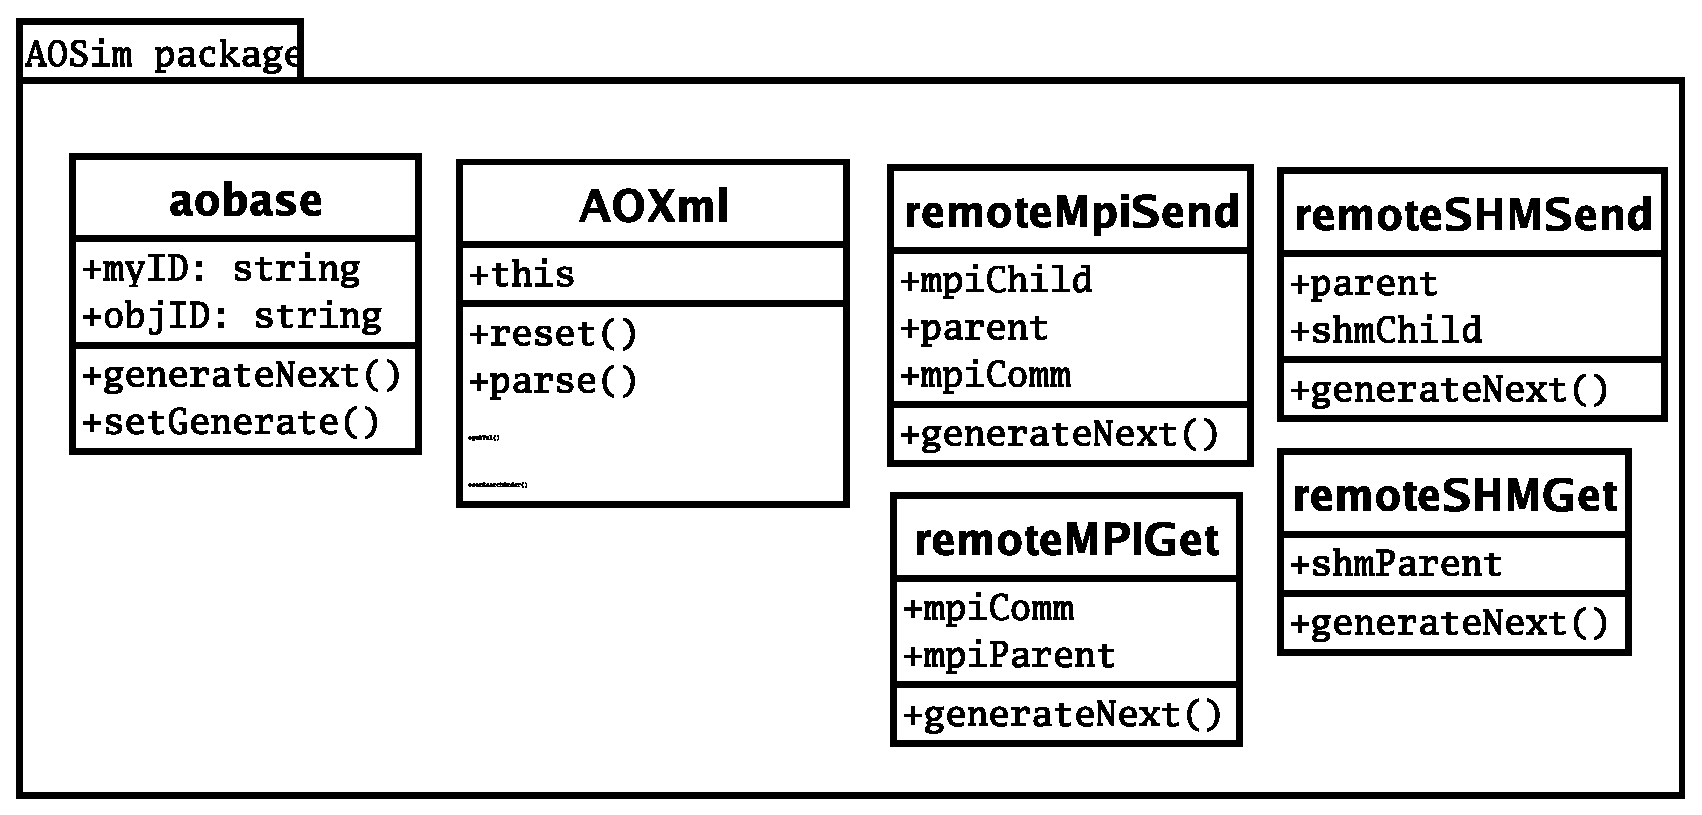
\includegraphics[width=15cm]{pics/baseClasses.eps}
\caption{A figure showing base classes provided in the simulation.}
\label{fig:baseclass}
\end{figure}

An example of the use of some of these modules is given in
Fig.~\ref{fig:usage}.  

\begin{figure}
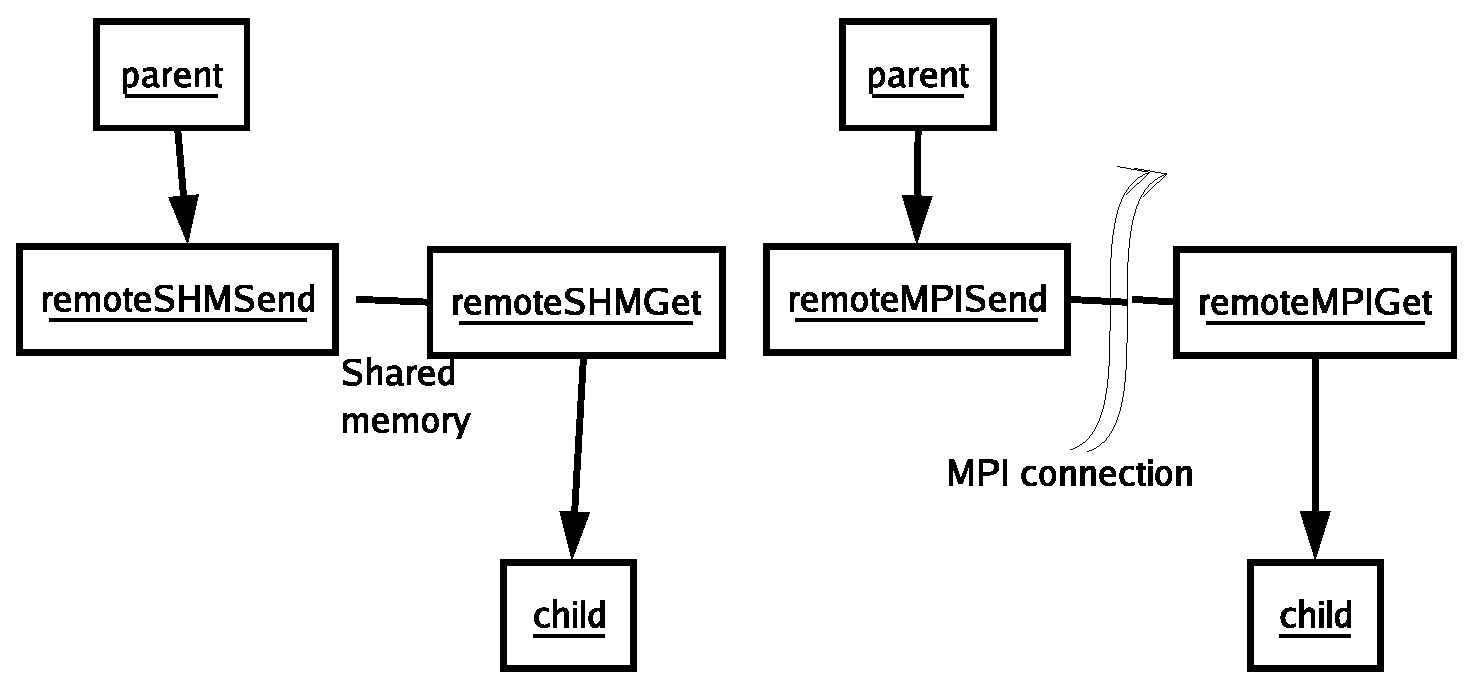
\includegraphics[width=10cm]{pics/baseClassUsage.eps}
\caption{A figure showing how framework objects can be used to
  interface between simulation modules.}
\label{fig:usage}
\end{figure}

\section{Working example}
A working example of a closed loop simulation is shown in
Fig.~\ref{fig:workingexample}, with the source code given in
appendix~\ref{app:src} (though this code may no longer work, and the
mkscrns and atmos modules have been superceeded).  The intention is
that similar source files may eventually be created using a GUI, which
will allow the user to connect modules together and specify where they
should run (separate nodes or processors).  There is an existing GUI
(paramgui.py) which can be used to create the XML parameter file, into
which all configuration parameters will be placed, allowing the file
to be regenerated or reloaded into the GUI when needed.

\begin{figure}
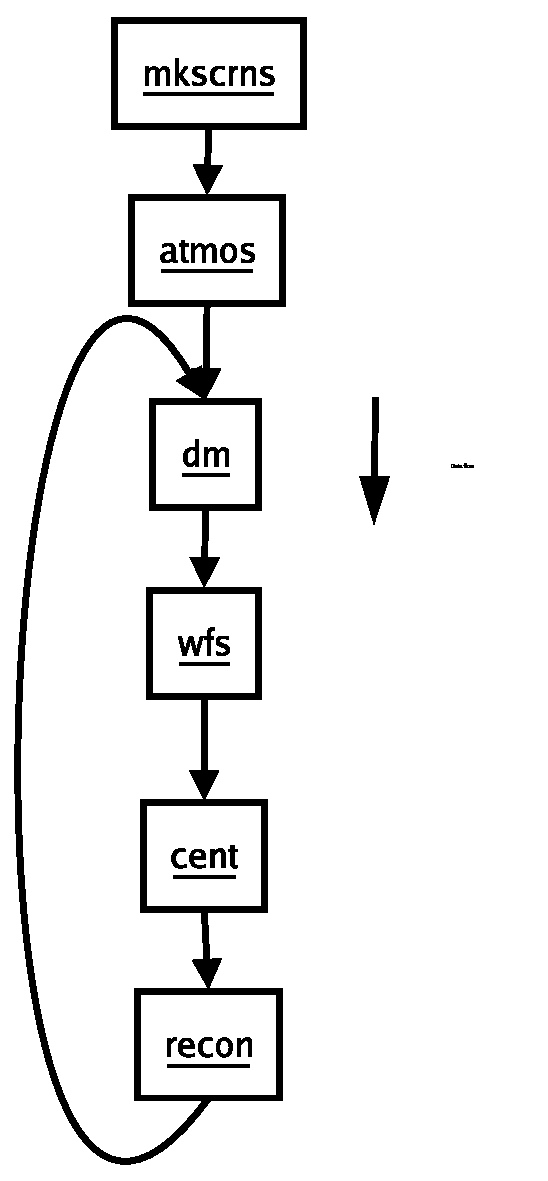
\includegraphics[height=8cm]{pics/simulation.eps}
\caption{An example of a closed loop AO simulation.}
\label{fig:workingexample}
\end{figure}

In this simulation, the mkscrns object generates a phase screen, which
is passed to the atmos module which produces the phase at the
telescope pupil for a given object at a given time.  The DM object
then places the effect of DM phase on this, and the wavefront sensor
is used to create an image.  Centroids are then computed, passed to a
reconstructor and then back the the deformable mirror.


\subsection{Multi threaded user modules}
If a user wishes to make a module multi-threaded (for example to run
as a background task, making sure that there is always data ready and
waiting), it is up to the user to ensure that data being accessed by
other objects doesn't changed.  The recommended way to ensure this is
to use a new data array for each data processing iteration.  However,
if these arrays are large (1-2GB), this could lead to memory
shortages, and so it is up to the user to be inventive in this
situation.  The use of multi-threaded user modules is not recommended
and should not be needed.

\section{Connecting to the simulation}
It is possible to connect to a running simulation, to obtain data, or
alter parameters ``on the fly'' (though this could be dangerous and is
not recommended unless you are sure about what you are doing).  When a
simulation is started, each process opens a TCP/IP listening socket on
a known port number (with a base number defined within the parameter
file and actual port numbers being equal to this plus the MPI rank).
Other processes can then connect to this socket, which behaves
somewhat like a (powerful) object broker, giving the connecting
process access to every variable and object within the simulation.

Typically, you will use this feature with the simctrl.py GUI (see
\citet{simctrlgui}) or the command line debugger, analyse.py (see
\citet{apidoc} for further details).  In brief, messages are sent to
this socket in the form of [command,code,tag,returnlist] using the
serialise library (Send function).  The listening process then reads
the socket.  The command word can be one of ``now'', ``cmd'', ``rpt'',
``rptN'' (integer N) or ``del''.  The code contains a string of code
to be executed using the python exec command.  This code will be
executed in the global object space of the simulation, so has access
to all objects, and is able to operate on them as desired by the user.
This means that the object broker can be used in a very flexible way,
as any code can be executed.  The returnlist (optional) contains a
list of variables to return.  If this list is not sent, all variables
defined within the exec call will be returned.  Further details of
this convention can be found in the API reference \citep{apidoc}.

This communication channel should be endian safe.  Since node 6 of the
XD1 is the only node with direct contact with the outside world
(though other nodes can be reached by automatic IP forwarding), any
data will be passed via node 6, which could give a performance loss if
care isn't taken.

\section{Module design}
The following are some rules which should be adhered to when making AO
simulation modules.  As these rules may be somewhat restrictive,
causing increased memory usage, or computation time, they are only
provided as a guide, and it is suggested that if a user is aware of
the consequences, they may bend some of these rules.  However, when
doing this, the user should provide a module object initialisation
switch (passed in the args dictionary when the module is instantiated)
which allows the object to be compliant (for naïve user usage) or
non-compliant (for memory/computation savings).
\subsection{Rules}
\begin{enumerate}
\item A module should always place output in a single numpy array
  object, called self.outputData.
\item A module should not alter the data it receives from the
  predecessor (found in self.parent.outputData).  It must make a copy
  if it wishes to do so.
\item A module should be documented using Python docstrings compatible
  with epydoc, so that the API reference manual can be kept up to
  date.
\item The module should inherit from base.aobase.  The module should
  (as a minimum) define a generateNext method.
\item A module should never use the ``from xxx import *'' method for
  importing.  Imports should always be by name.
\item A module should have a forGUISetup argument in the \_\_init\_\_
  method which can be used when the module is just required for
  querying, and not to do any computation (for example, a GUI may use
  this to determine data sizes etc.).  If this flag is set, the object
  must contain an outputdata object which is a Python tuple of (output
  data array dimensions, output data array datatype), for example,
  self.outputdata=((1024,1024), numpy.float32).  This can then be
  used for instantiating MPI or SHM objects as well as the GUI, simply
  by querying the value of the instantiated object's outputdata
  object.
\item A module can have a simctrlXML method, which takes a single
  string arguement, and returns a string which can be placed into an
  XML file for GUI simctrl.py usage.  The input for this method is the
  name of the object created, and should be used within the method.
  This method will be automatically called at simulation start-up, and
  is a nice way of allowing a user to get simulation control without
  having to write their own simctrl.xml file.
\end{enumerate}
These rules are not complete, and may be added to at any time when I
remember what I've missed.

\subsection{Modules returning multiple data outputs}
If you wish to create a module which has multiple outputs (i.e.\
computes several different things), you can do this as follows.
First, calculate how much data storage is required for all the
outputs, and create a one-dimensional numpy byte-array large enough
to hold all this, and assign it to \texttt{self.outputData} (this is
the storage array).  Then use
the \texttt{util.arrayFromArray} function to sub-divide this
array into the different output arrays that you require, and write
your results to these arrays.  You can then
split this data output by using different instances of
\texttt{base.splitOutput} objects, each indexing a different part of
the storage array.  These \texttt{splitOutput} modules can then be
treated by other modules as generating the required data.  The
\texttt{arrayFromArray} function takes three arguements which are a
contiguous array to be subdivided, the shape of the new array, and the
datatype of the new array.  An additional byte offset can also be
specified if required.  It then returns an array with the given type
and shape which shares its data region with the original array, i.e.\
no new memory is allocated.

\subsubsection{Example}
If I have a module which produces a 1-D 64 bit floating point array
with 500 elements, a 2-D 32 bit integer array with (10,10) elements
and a 2-D byte array with (1000,1000) elements, I could do the
following:

Note, this example is now out of date, since we use numpy instead.  In
this case, please use util.arrayFromArray.arrayFromArray in the same way.

\begin{verbatim}
#In my science object:
self.outputData=numpy.zeros((500*8 + 10*10*4 + 1000*1000*1,),numpy.uint8)

self.oneDArr=util.arrayFromArray.arrayFromArray(self.outputData[:500*8],(500,),numpy.float64)
self.intArr=util.arrayFromArray.arrayFromArray(self.outputData[500*8:500*8+10*10*4],(10,10),numpy.int32)
self.byteArr=util.arrayFromArray.arrayFromArray(self.outputData[500*8+10*10*4:500*8+10*10*4+1000*1000],
                                       (1000,1000),numpy.int8)

#now do the calculations, writing results to oneDArr, intArr and
 byteArr.

########
#Now, in your simulation definition file, you would use:
myobj=science.myobj(parent,config,...)

getOneDArr=base.splitOutput.splitOutput(myobj,config,args={"startOffset":0,"shape":(500),
                                                           "dtype":"d"})
getIntArr=base.splitOutput.splitOutput(myobj,config,args={"startOffset":500*8,"shape":(10,10),
                                                           "dtype":"i"})
getByteArr=base.splitOutput.splitOutput(myobj,config,args={"startOffset":500*8+10*10*4,
                                                           "shape":(1000,1000),"dtype":"b"})

#The getOneDArr, getIntArr and getByteArr objects now contain the
#different data arrays that you require.
\end{verbatim}

Note that it is necessary to create the arrays like this because all
objects are expected to place their outputs in the
\texttt{self.outputData} array, so that they can be treated in a
uniform way by MPI, SHM and other objects.  However, the flexibility
of the framework also allows multiple outputs to be created in this
way.  Note, that this does not require any additional memory
allocations, i.e.\ the arrays provided by the \texttt{splitOutput}
objects share the same memory as the original array.

\section{Running a simulation}
There are various command line switches that can be used to run a
simulation.  These are documented more fully in the dummiesGuide and include:

\begin{enumerate}
\item -h or --help to display a help message (including an up to date
  list of command line arguments).
\item --start-paused to place the simulation in an initial paused
  state.
\item --param-file=FILENAME to specify a parameter file name (the
  default is params.xml).
\item --batchno=INT to specify an integer batch number (which means it
  will read variables corresponding to this batch from the param file)
\item --id=STRING to specify an ID for the simulation.
\item --iterations=N to specify the number of iterations the simulation
  is run for (the default is infinity if not specified in the
  parameter file).
\item --param=''python text string'' to change a parameter on the fly.
\end{enumerate}
If you use the simsetup GUI, the first line of the file will contain a
comment, with a suggestion of how to execute the simulation.

To be able to run a simulation such that it doesn't quit when you log
out, either run it preceeded by nohup (e.g. nohup python sim.py) or
(to apply this to a running simulation), suspend the simulation
(Ctrl-z), send it to background (bg) and then use the bash command
disown -h.  Your simulations will now continue running when you log out. 

\subsection{Considerations}
There are a number of considerations when setting up a simulation.
Make sure you understand the labelling of optical paths, and how this works.

\section{XML file notation}
\label{sect:paramfile}
\subsection{Parameter file}
The parameter file begins with an XML compliant line \texttt{<?xml
version="1.0"?>}.  Following this, there must be an \texttt{<aosim>}
tag, within which all parameters and schema information are defined.
A \texttt{<schema>} tag is used to define the schema part of the
parameter file, and is used to define how simulation objects are
connected together and instantiated.  This has not yet been fully
implemented, but it is intended that eventually, this schema section
will be used to write a python file which can then be run as the
simulation.  The parameter file will therefore be all that is required
for a working simulation.

\texttt{<module>} tags are then used to order the variables.  The
module tag must have an attribute ``name'', the value of which can be
``globals'', or that of a specific simulation object.  The name of the
module must be identical to the \texttt{objID} class variable within
the science object to which it applies.  Typically, this will just be
the name of the file in which the object is placed without the
trailing \texttt{.py}.  However, if during instantiation of the
object, an identification string is passed in the \texttt{args}
dictionary with a key of \texttt{"idstr"}, then the corresponding
value will be appended to the module name, after a ``\_'', for example
\texttt{"idstr":''XXX''} would give a module name of
\texttt{mymodule\_XXX}.  This allows the user to differentiate between
objects of the same type, within the parameter file, providing for
example, different source angles or magnitudes for different stars.

Within these \texttt{<module>}, \texttt{</module>} tags, there will be
a \texttt{<variables>}, \texttt{</variables>} set of tags which
enclose instances of \texttt{<var>}.  The \texttt{<var>} tags have
attributes ``name'', ``type'', ``value'' and optionally ``comment''.
The value of the ``name'' attribute must be the variable name.  The
value of ``type'' can be one of ``f'' (floating point), ``i''
(integer), ``numpy'' (array), ``copy'', ``list'', ``code'', ``eval''
or ``string''.  The value of value is then converted to a python
object depending on type.  Table~\ref{table:conversiontable} shows the
method used to convert the value string into a Python object.

\begin{table}
\begin{tabular}{|l|l|l|}\hline
Type & Conversion method & Comment/Example\\ \hline
i & int(value) & e.g.\ ``10''\\ \hline
f & float(value) & e.g.\ ``5.998''\\ \hline
numpy & eval(value) & e.g.\ ``numpy.zeros((10,20), 'i')''\\ \hline
copy & eval(value) & e.g.\ ``this.globals.wfs\_n''\\ \hline
list & eval(value) & e.g.\ ``[1,2.09,'hello']''\\ \hline
code & exec(value) & e.g.\ ``import math ; name=math.cos(10)''\\
&& The value of ``name'' will be obtained from\\
&& the dictionary created by the exec call.\\ \hline
eval & eval(value) & e.g.\ ``5*10.0'' \\ \hline
string & value & e.g.\ ``Hello''\\ \hline
\end{tabular}
\caption{A table showing how the type defined in the parameter file is
  converted to a python type}
\label{table:conversiontable}
\end{table}

Within this parameter file, the name ``this'' can be
used to reference other variables already defined (when an exec or
eval call is used).  The ``copy'' example in
table~\ref{table:conversiontable} gives an example of this.

An example parameter file is given in appendix~\ref{app:paramfile}.

\subsection{GUI definition file}
A GUI definition file can be used with the simulation control GUI to
present the user with a selection of commands relevant to a given
simulation.  Further details of the format of this file are given in
\citet{simctrlgui}.  

\section{The GUI suite}
What follows are some suggestions and thoughts about how the GUI
should be implemented, and what features is should have.
Additionally, requirements for the science modules to operate with the
GUI suite are also included.

\subsection{Setup GUI}
The setup GUI is used to link modules together, and produce a script
which when run will run the simulation, and is currently vapourware.
The GUI must therefore be able to:

\begin{itemize}
\item Import new modules
\item Allow the user to link modules together legally (knowing what they
produce and expect to receive)
\item Give the user control over where specific modules are run (node
  and processor)
\end{itemize}

These requirements mean that detailed knowledge of any given class
object will be required.  The most sensible way to obtain this
knowledge seems to be to instantiate an object, and so obtain access
to it's internals.  However, instantiation of some objects (for
example a phase screen generator object) may require large amount of
memory, or processing time.  This is not desirable when setting up the
simulation, and so it is suggested that each object can be
instantiated with a ``forGUISetup'' flag set to one
(with a default of zero).  When this flag is set, the object will only
instantiate the bare minimum required by the GUI.  The object can then
be queried for parameters required and default values, as well as for
data input and output requirements.

A call to the object's getInputType() and getOutputType() methods will
return information about the input and output data required by the
object in a yet-to-be-determined format (see aobase.py file for latest
development).  The GUI can then use this information to determine
whether the object has compatible predecessors and successors.
Such a format may be a type object with variables for type
(e.g. IntType, arrayType, * for any type), dimensions (with a negative
dimension meaning anything) etc, or a list of such type objects if
several are allowed.  The type object will also have a description
variable, which gives a text description of what the inputs and
outputs should be, e.g. ``wfs data''.  If these descriptions do not
match between two connected modules, the user is warned, but the
connection is still allowed.  However if the type and dimensions do
not match, the connection is not allowed.

It is up to the creator of the module to ensure that the getParams(),
getInputType() and getOutputType() methods are kept up to date when
changes to the module are made.

A call to the object's getInitArgs() will return a dictionary of the
expected parameters which can be used when initialising the object,
with a brief description and default value (if the default value does
not exist, it is not an optional parameter).  This dictionary can be
used by the GUI to give the user choices when producing the
simulation.

A call to the object's plottable() will return a XML string to be
placed into the XML file used by the simctrl.py GUI for simulation
control.  This XML string contains the default settings which will be
displayed and used in the simctrl.py GUI for displaying data and
controlling the simulation.  The XML string will appear as GUI
buttons, which, when pressed will send the corresponding command over
the socket to the simulation process (which should then return
corresponding data).  Within this command, the string \$OBJ can be
replaced by the objects name once the object is generated.

\subsection{Parameter GUI}
The paramgui.py GUI should be used to alter simulation parameters, and
the user should be able to specify whether this is globally, or local
to a specific class object or even object instance.  For any
unspecified parameters, if a default value is not requested in the
simulation code, an error will be raised.  The paramgui.py GUI is able
to parse a simulation python module, and determine which parameters
need adding, and also can make use of a simulation object getParams()
method if this exists.

The user will specify the parameters in exactly the way in which they
will be placed into the parameter file, and so this allows for some
parameters to depend on others, and be generated on the fly.  The
getParams() method should not be used during simulation, as all
parameters should be defined within the parameter file.

A call to the object's getParams() method will return a dictionary of
{``paramName'': (defaultValue,comment)...}.  The GUI will
display this list to the user, and allow them to set values (local or
global) which will be stored within the XML parameter file for the
simulation.  The parameter GUI is discussed in more detail in
\citet{simparamgui}. 


\subsection{Simulation control GUI}
The simulation GUI has been designed to allow complete control of the
AO simulation, and provide feedback such as plots and data.  The GUI
is capable of displaying any data required and the user is able to add
new buttons to implement new displays (i.e. sending a new command to
the simulation, and so obtaining data which has not been displayed
before).  The simulation GUI is discussed in more detail in
\citet{simctrlgui}.


\subsection{Module checking}
A science module can be checked for compatibility with these
requirements using the checkModule.py file found in the
util/ directory.  This will check that a given simulation object has
valid getParams, getInitArgs, getInputType and getOutputType
methods.  Further tests may be added at a later date.   This hasn't
been tested for a long time, so may not work...

To use this facility, make sure you are in the same directory as your
module source code.  If this module is called mkscrns.py and contains
an object called Mkscrns, you would test by calling 
\begin{verbatim}
python path\_to\_cvs\_root/aosim/util/checkModule.py mkscrns Mkscrns
\end{verbatim}
Error (or success) messages will then be printed.
It is wise to make sure your module conforms to this standard before
using it with the GUI.  However, this check does not guarantee that
your module is compatible with the simulation, rather it increases the
chances of it being so.


\section{Available and required libraries}
There are a number of libraries that are available to a simulation
user, and which are required for the simulation to function.  These
libraries allow the user to develop their own modules, or analyse data
from current modules with ease.

They include
\begin{description}
\item[Gist] Graphical plotting library (probably not any more).
\item[Pylab] Graphical plotting library.
\item[FFTW 2] Fourier transform library version two (using custom wrappers).
\item[FFTW 3] Fourier transform library version three (using custom wrappers).
\item[Scientific Python] Scientific computing library, including MPI
  communication among other things.
\item[pygtk] Graphical User Interface library.
\item[PIL] Python imaging library (probably not anymore).
\item[pygsl] Wrappers for gsl (Gnu scientific library).
\item[Numeric] Array manipulation library (depreciated, hopefully not needed now)
\item[numpy] Array manipulation library.
\item[scipy] Scientific library
\item[epydoc] Latex documentation library (not needed if you don't
  want to generate the API documentation)
\end{description}

Information about all of these libraries is available on the web.
Other libraries can be made available upon request.

\section{Simulation input and output}
\subsection{Simulation input parameters}
The simulation input parameters should be stored in an XML file, as
described in section~\ref{sect:paramfile}.  If large amounts of data
(e.g.\ image data etc.) are required as part of this, then a file
(e.g.\ a FITS file) containing this information should be placed in
the same directory as the parameter file, and the parameter file
should then be used to load this information into a Python object,
which is then made available to the simulation.  The flexibility of
the parameter file format allows this.

\subsection{Simulation results}
The output from a simulation can be saved in many ways.  However, the
standard way to save information and data is using a FITS file.  For
image data, a FITS image array should be used, and other data should
be stored in FITS tables.  The header of the FITS file should include
the creation time and date, user name, simulation file and parameter
file, simulation iteration number, and any other relevant information.
If a module can (but does not necessarily) output data such as timing
information or the variance of some quantity or the flux, or even its
configuration such as number of lenslets, then it can be appended to
some end-of-run FITS data file which holds all the necessary data for
the simulation run. This then can be analysed at some later stage
without needing the actual simulation parameter file.  This is useful
when you archive data from previous runs (for testing) or when you
give the data to someone else (person A runs the sim, persons A and B
analyse the data).  As an alternative file format when a FITS file is
not appropriate, the user can pickle parts or all of the simulation.

\section{Advanced and new features}
\subsection{Reuse of module memory}
This is termed resource sharing - any module that can share its
resources without affecting results can be made so share it with other
similar modules.

This will allow a module to be called more than once during an
iteration, and each time will use different parameters, so creating a
different output, whilst at the same time using the same memory
arrays.  This may be essential for ELT scale simulations, and also
decreases simulation runtime.  For example, take the infinite
atmosphere module.  If you are observing in several different
directions, you need several different atmosphere modules, each
containing an array of phase values for each atmospheric layer.  These
phase arrays could be upto half a GB each, and so memory soon becomes
short when using a multiply layer system, observed in multiple
directions.  The solution is to have a single atmospheric module, to
which all the different DM/science/centroid modules connect for the
different directions.  The atmospheric module would be called for the
first direction, and then the necessary DM etc modules would then be
called.  Then, in the same simulation iteration, the atmospheric
module would be called for the second direction.  The necessary
(different) DM etc modules would then be called.  This would repeat
until all directions had been computed for this node.  The next
simulation iteration would then start.

This can be set up in the simsetup GUI.  Note, centroid objects
shouldn't be shared unless you make a copy of the output immediately
after they are called (otherwise this will be overwritten before the
reconstructor sees it).

Inf\_mksrcns and recon objects are not resource sharing.  Plus, the
memory requirements of these can be smaller.

\subsection{Multithreading}
The advent of multicore processors means that true multi-threading can
have an advantage.  However, Python allows only one thread to be
executed at a single time, due to the global interpreter lock.  To use
Python on multicore processors would therefore require MPI or
something similar, which may reduce efficiency.  A better approach
would be to code in C the algorithms that could benefit, and have
these C algorithms multithreaded.  So, Python would make the C call,
which would then execute in a multithreaded fashion, before waiting
for thread completion and returning to Python.  This currently works
for the centroid module.  Other modules will be updated in due course.

\subsection{Grouping}
Similar atmospheric paths can be grouped together in the simsetup GUI,
which allows simulation creation to be simplified.

\subsection{Data sharing}
There is now a facility using config.post and config.postGet methods
to share data around the simulation.  This should be treated as a rare
occurance as will be fairly slow (TCP/IP), but is useful for passing
some rarely calculated results between modules (eg covariance matrices
etc).

\subsection{Stopping a simulation cleanly}
When running a multi-process (MPI or SHM) simulation, to stop the
simulation cleanly, the following procedure should be followed.  This
is because simply pressing the stop button means that the stop may
occur when different processes are in different iterations (some may
be blocked waiting on an MPI event).  So, first, pause all
processes.  For the processes that are paused successfully (print a
paused message or have ctrl.paused=1), advance these by 1 iteration.
You should then see that all processes are paused at the next
iteration (including those that weren't paused before).  The
simulation is now in synchronisation, and so can be stopped.  Press
the stop button for all processes.

\section{Conclusion}
An overview of the AO simulation has been given.  If any parts of this
documentation have been unclear, or you would like to see extra
documentation added, please either edit the file yourself, or ask
someone else to (and remember to commit the changes).  Happy
simulating!

\section{Work to be done: TODO}
There are several things that still need to be done.
\begin{enumerate}
\item Reuse of module memory - done
\item More FPGA code (or maybe not) - no
\item Cell processor use - done
\item Porting intensive parts of Python code to C - ongoing
\item Creating C code with multiple threads (for use on multi-core
  systems), the best option would be to has a user definable number of
  threads, which defaults to the number of available CPU cores (from
  /proc/cpuinfo or equivilent).  Ongoing.
\end{enumerate}


\appendix
\section*{Appendix 1: Sample code listing}
\label{app:src}
WARNING: this code listing may be out of date.  See the examples
within the simulation CVS for up-to-date versions.  In particular,
look in examples/test1/ at files simple.py and params.xml.

\begin{verbatim}
import science.mkscrns
import science.atmos
import science.el_dm
import science.wfs
import science.cent
import science.el_recon
import util.Ctrl
import numpy
ctrl=util.Ctrl.Ctrl(globals=globals(),debug="ctrl")
#set up the science modules
Mkscrns=science.mkscrns.mkscrns(None,ctrl.config)
Atmos=science.atmos.atmos(Mkscrns,ctrl.config)
Dm=science.el_dm.dm({"atmos":Atmos},ctrl.config)
Wfs=science.wfs.wfs(Dm,ctrl.config,args={"fpprecision":32})
Cent=science.cent.cent(Wfs,ctrl.config)
Recon=science.el_recon.recon(Cent,ctrl.config)
Dm.parent["recon"]=Recon
execOrder=[Mkscrns,Atmos,Dm,Wfs,Cent,Recon]
ctrl.mainloop(execOrder)#start the main simulation loop
\end{verbatim}

\section*{Appendix 2: Sample parameter file}
\label{app:paramfile}
This is an example of a sample (incomplete) parameter file.  Please
see example/test1/params.xml instead.

\begin{verbatim}
<?xml version="1.0"?>
<aosim>
<author name="Francois Assemat"/>
<created date="01072005"/>
<module name="globals">
<variables>
<var name="fpDataType" type="code">
import numpy
fpDataType=numpy.float64
</var>
<var name="tstep" value="0.005" type="f" comment="time step"/>
<var name="testrunport" type="i" value="9000" comment="port number for
connections"/>
<var name="npup" type="i" value="64"/>
<var name="itersPerPhaseScreen" type="i" value="1000" 
     comment="Number of iterations per mkscrn phase screen"/>
<var name="ntel" type="copy" value="this.globals.npup"/>
<var name="pupil" type="code" comment="Telescope pupil function">
import util.tel
pupil=util.tel.Pupil(this.globals.npup,this.globals.ntel/2,
             this.globals.ntel/2*this.globals.telSec/this.globals.telDiam)
</var>
</variables>
</module>

<module name="pyramid_1">
<variables>
<var name="xy" type="i" value="10"/>
</variables>
</module>
<module name="pyramid_2">
<variables>
<var name="xy" type="i" value="11"/>
</variables>
</module>
<module name="pyramid">
<variables>
<var name="size" type="i" value="10"/>
<var name="xy" type="eval" value="max(this.pyramid_1.xy,this.pyramid_2.xy)"/>
</variables>
</module>
</aosim>
\end{verbatim}

\pagebreak
\bibliography{references}


\printindex
\end{document}
